\documentclass[a4paper,12pt]{report}

\usepackage[T2A]{fontenc}
\usepackage[utf8]{inputenc}
\usepackage[english,ukrainian]{babel}
\usepackage{amsmath}
\usepackage{ragged2e}
\usepackage{graphicx}
\graphicspath{ {./} }

\usepackage{titlesec}
\titleformat{\section}[block]{\Large\bfseries\filcenter}{}{1em}{}
\titleformat{\subsection}[block]{\bfseries\filcenter}{}{1em}{}
\titleformat{\chapter}[block]{\Huge\bfseries\filcenter}{}{1em}{}


\author{Кирило Байбула Аленович}
\title{ГЕНЕРУВАННЯ ПСЕВДОВИПАДКОВИХ ЧИСЕЛ}

\begin{document}

  \begin{titlepage}
    \begin{center}
        \Large
        \textbf{Київський національний університет імені Т.Шевченка}
        \vspace{5cm}

        \Huge
        \textbf{Звіт}

        \LARGE
        До лабораторної роботи №1
        \vspace{0.5cm}

        \textbf{ГЕНЕРУВАННЯ ПСЕВДОВИПАДКОВИХ ЧИСЕЛ}
        \vfill
    \end{center}

    \begin{FlushRight}
        Кирило Байбула Аленович\\
        Групa К-21\\
        Факультету комп’ютерних наук \\
        та кібернетики
    \end{FlushRight}

      \vspace{0.5cm}

    \begin{center}
      \textbf{Київ} \\
      2021
    \end{center}

  \end{titlepage}
  \clearpage

  \chapter*{МЕТА}

Написати програму, що реалізує десять генераторів псевдовипадкових чисел.
Кожний генератор викликати за допомогою меню, яке реагує на ввід цілого числа:
1, \ldots, 10. Згенерувати послідовність псевдовипадковіх чисел, яка має якнайдовший
період (не менше 100). \par
Побудувати гістограму, яка ілюструє розподіл чисел на інтервалах \mbox{[0;1]} (для
нормального розподілу), \mbox{[-3;3]} (для нормального розподілу), \mbox{[0; 100]} – для решти
розподілів. Гістограму подати у вигляді таблиці. Наприклад, для рівномірного
розподілу вона виглядатиме приблизно так. Частота обчислюється як дріб,
чисельником якого є кількість потраплянь випадкових чисел в певний інтервал, в
знаменником – повна кількість згенерованих чисел.
\begin{table}[ht]
\centering % used for centering table
\begin{tabular}{c c} % centered columns (4 columns)
  Інтервал & Частота \\\relax
  [0.1;0.2] & 0.15 \\\relax
  [0.2;0.3] & 0.1 \\\relax
  [0.3;0.4] & 0.12 \\\relax
  [0.4;0.5] & 0.15 \\\relax
  [0.5;0.6] & 0.05 \\\relax
  [0.6;0.7] & 0.08 \\\relax
  [0.7;0.8] & 0.16 \\\relax
  [0.8;0.9] & 0.04 \\\relax
  [0.9;1.0] & 0.1
\end{tabular}
\label{table:nonlin} % is used to refer this table in the text
\end{table}

Генератори псевдовипадкових чисел, як правило, породжують ціле число X, яке
лежить в інтервалі від 0 до деякого заздалегідь заданого числа m. Тому дійсні
псевдовипадкові числа, рівномірно розподілені між 0 і 1, обчислються за формулою \[U = X/m\]
\clearpage

\chapter*{МЕТОДИ ГЕНЕРУВАННЯ}
\section{Методи генерування рівномірно розподілених чисел}
\subsection{Лінійний когyруентний}
\[X_{n+1}=(aX_{n} + c )\mod m,\]
\[U_{n+1} = X_{n+1}/m, n\ge0, \]

де $m$ – модуль, $m > 0$, $a$ – множник, $0 \le a < m$, $c$ – приріст, $0 \le с < m$, $X_{0}$ – початкове
значення, $0 \le X_{0} < m$.

Таблиця інтервалів та частот попадання чисел для лінійного конгурентного методу при $10,000,000$ псевдовипадково знегеровних чисел:

\begin{table}[ht]
\centering % used for centering table
\begin{tabular}{c c} % centered columns (4 columns)
  Інтервал & Частота \\\relax
  [0.0; 0.1] & 0.10 \\\relax
  [0.1; 0.2] & 0.10 \\\relax
  [0.2; 0.3] & 0.10 \\\relax
  [0.3; 0.4] & 0.10 \\\relax
  [0.4; 0.5] & 0.10 \\\relax
  [0.5; 0.6] & 0.09 \\\relax
  [0.6; 0.7] & 0.10 \\\relax
  [0.7; 0.8] & 0.10 \\\relax
  [0.8; 0.9] & 0.10 \\\relax
  [0.9; 1.0] & 0.10
\end{tabular}
\end{table}
Фотографія гістограмми програми у стандартний поток виводу:
\begin{center}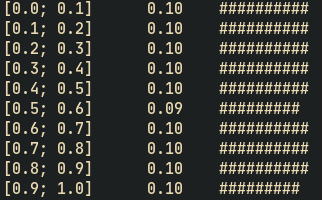
\includegraphics[scale=0.5]{linear}\end{center}

\subsection{Квадратичний конгруентний метод}
\[X_{n+1}=(dX_{n}^{2}  + aX_{n} + c )\mod m,\]
\[U_{n+1} = X_{n+1}/m, n\ge0, \]

Таблиця інтервалів та частот попадання чисел для квадратичного конгруентного методу при $10,000,000$ псевдовипадково знегеровних чисел:

\begin{table}[ht]
\centering % used for centering table
\begin{tabular}{c c} % centered columns (4 columns)
  Інтервал & Частота \\\relax
  [0.0; 0.1] & 0.12 \\\relax
  [0.1; 0.2] & 0.09 \\\relax
  [0.2; 0.3] & 0.12 \\\relax
  [0.3; 0.4] & 0.08 \\\relax
  [0.4; 0.5] & 0.11 \\\relax
  [0.5; 0.6] & 0.16 \\\relax
  [0.6; 0.7] & 0.08 \\\relax
  [0.7; 0.8] & 0.11 \\\relax
  [0.8; 0.9] & 0.07 \\\relax
  [0.9; 1.0] & 0.06
\end{tabular}
\end{table}
Фотографія гістограмми програми у стандартний поток виводу:
\begin{center}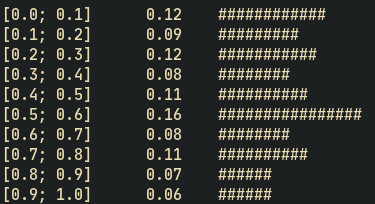
\includegraphics[scale=0.5]{square}\end{center}


\subsection{Числа Фібоначчі}
\[X_{n+1}=(X_{n}  + X_{n-1})\mod m, n \ge 0\]
\[U_{n+1} = X_{n+1}/m, n\ge0, \]

Таблиця інтервалів та частот попадання чисел для Чисел Фібоначчі при $10,000,000$ псевдовипадково знегеровних чисел:

\begin{table}[ht]
\centering % used for centering table
\begin{tabular}{c c} % centered columns (4 columns)
  Інтервал & Частота \\\relax
  [0.0; 0.1] & 0.11 \\\relax
  [0.1; 0.2] & 0.10 \\\relax
  [0.2; 0.3] & 0.10 \\\relax
  [0.3; 0.4] & 0.10 \\\relax
  [0.4; 0.5] & 0.09 \\\relax
  [0.5; 0.6] & 0.10 \\\relax
  [0.6; 0.7] & 0.11 \\\relax
  [0.7; 0.8] & 0.10 \\\relax
  [0.8; 0.9] & 0.09 \\\relax
  [0.9; 1.0] & 0.10
\end{tabular}
\end{table}
Фотографія гістограмми програми у стандартний поток виводу:
\begin{center}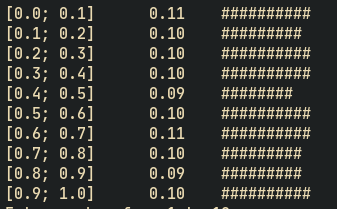
\includegraphics[scale=0.5]{fibb}\end{center}


\subsection{Обернена конгруентна послідовність}
\[X_{n+1}=(aX_{n}^{-1}  + c)\mod m, n \ge 0\]
\[U_{n+1} = X_{n+1}/m, n\ge0, \]

Таблиця інтервалів та частот попадання чисел для Оберненого методу при $10,000,000$ псевдовипадково знегеровних чисел:

\begin{table}[ht]
\centering % used for centering table
\begin{tabular}{c c} % centered columns (4 columns)
  Інтервал & Частота \\\relax
  [0.0; 0.1] & 0.10 \\\relax
  [0.1; 0.2] & 0.10 \\\relax
  [0.2; 0.3] & 0.10 \\\relax
  [0.3; 0.4] & 0.10 \\\relax
  [0.4; 0.5] & 0.10 \\\relax
  [0.5; 0.6] & 0.10 \\\relax
  [0.6; 0.7] & 0.10 \\\relax
  [0.7; 0.8] & 0.10 \\\relax
  [0.8; 0.9] & 0.10 \\\relax
  [0.9; 1.0] & 0.10
\end{tabular}
\end{table}
Фотографія гістограмми програми у стандартний поток виводу:
\begin{center}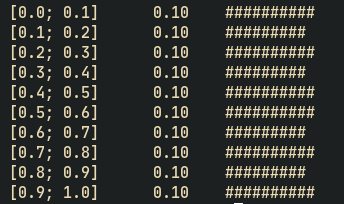
\includegraphics[scale=0.5]{inverse}\end{center}

\subsection{Метод об’єднання}
\[Z_{n}=(X_{n}  - Y_{n})\mod m, n \ge 0\]
\[0 \le X_{n} < m, 0 \le Y_{n} < m' <= m\]
\[U_{n+1} = Z_{n+1}/m, n\ge0, \]

Таблиця інтервалів та частот попадання чисел для Методу об’єднання при $10,000,000$ псевдовипадково знегеровних чисел:

\begin{table}[ht]
\centering % used for centering table
\begin{tabular}{c c} % centered columns (4 columns)
  Інтервал & Частота \\\relax
  [0.0; 0.1] & 0.10 \\\relax
  [0.1; 0.2] & 0.10 \\\relax
  [0.2; 0.3] & 0.10 \\\relax
  [0.3; 0.4] & 0.10 \\\relax
  [0.4; 0.5] & 0.10 \\\relax
  [0.5; 0.6] & 0.10 \\\relax
  [0.6; 0.7] & 0.10 \\\relax
  [0.7; 0.8] & 0.10 \\\relax
  [0.8; 0.9] & 0.10 \\\relax
  [0.9; 1.0] & 0.10
\end{tabular}
\end{table}
Фотографія гістограмми програми у стандартний поток виводу:
\begin{center}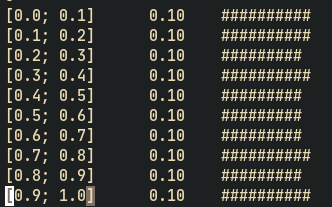
\includegraphics[scale=0.5]{union}\end{center}

\section{Методи нормального розподілу}

\subsection{Метод об’єднання}
\[X_{n} = m + (sum - 6) \sigma ,\]
де m – медіана, $\sigma$ – дисперсія, sum – сума дванадцяти випадкових чисел, рівномірно
розподілених на інтервалі [a, b]. Якщо [a, b] = [0; 1], то m = 0, а $\sigma$ = 1. Правило 3-сігма
стверджує, на проміжку [m–3$\sigma$, m+3$\sigma$] міститься 99,7\% всіх випадкових чисел, що
мають розподіл N(m,$\sigma$2 ). Отже для побудови гістограми розподілу N(0,1) достатньо
обмежитись інтервалом [-3;3].
Таблиця інтервалів та частот попадання чисел для Правил Трьох сігма при $10,000,000$ псевдовипадково знегеровних чисел:

\begin{table}[ht]
\centering % used for centering table
\begin{tabular}{c c} % centered columns (4 columns)
  Інтервал & Частота \\\relax
[-3.0; -2.4] & 0.01 \\\relax
[-2.4; -1.8] & 0.03  \\\relax
[-1.8; -1.2] & 0.07 \\\relax
[-1.2; -0.6] & 0.16 \\\relax
[-0.6; +0.0] & 0.23 \\\relax
[+0.0; +0.6] & 0.22 \\\relax
[+0.6; +1.2] & 0.18 \\\relax
[+1.2; +1.8] & 0.08 \\\relax
[+1.8; +2.4] & 0.02 \\\relax
[+2.4; +3.0] & 0.01
\end{tabular}
\end{table}
Фотографія гістограмми програми у стандартний поток виводу:
\begin{center}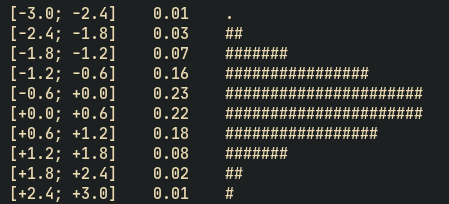
\includegraphics[scale=0.5]{sigma}\end{center}

\subsection{Метод полярних координат}
Таблиця інтервалів та частот попадання чисел для Методу полярних координат при $10,000,000$ псевдовипадково знегеровних чисел:

\begin{table}[ht]
\centering % used for centering table
\begin{tabular}{c c} % centered columns (4 columns)
  Інтервал & Частота \\\relax
[-3.0; -2.4] & 0.01 \\\relax
[-2.4; -1.8] & 0.03  \\\relax
[-1.8; -1.2] & 0.07 \\\relax
[-1.2; -0.6] & 0.17 \\\relax
[-0.6; +0.0] & 0.24 \\\relax
[+0.0; +0.6] & 0.23 \\\relax
[+0.6; +1.2] & 0.14 \\\relax
[+1.2; +1.8] & 0.08 \\\relax
[+1.8; +2.4] & 0.03 \\\relax
[+2.4; +3.0] & 0.01
\end{tabular}
\end{table}
Фотографія гістограмми програми у стандартний поток виводу:
\begin{center}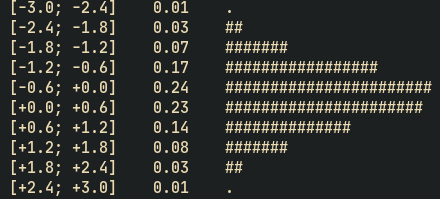
\includegraphics[scale=0.5]{polar}\end{center}



\subsection{Метод співвідношень}
Таблиця інтервалів та частот попадання чисел для Методу полярних координат при $10,000,000$ псевдовипадково знегеровних чисел:

\begin{table}[ht]
\centering % used for centering table
\begin{tabular}{c c} % centered columns (4 columns)
  Інтервал & Частота \\\relax
[-3.0; -2.4] & 0.01 \\\relax
[-2.4; -1.8] & 0.03  \\\relax
[-1.8; -1.2] & 0.07 \\\relax
[-1.2; -0.6] & 0.18 \\\relax
[-0.6; +0.0] & 0.21 \\\relax
[+0.0; +0.6] & 0.22 \\\relax
[+0.6; +1.2] & 0.18 \\\relax
[+1.2; +1.8] & 0.06 \\\relax
[+1.8; +2.4] & 0.02 \\\relax
[+2.4; +3.0] & 0.01
\end{tabular}
\end{table}
Фотографія гістограмми програми у стандартний поток виводу:
\begin{center}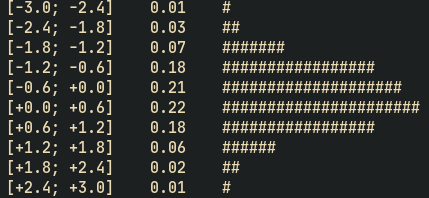
\includegraphics[scale=0.5]{correl}\end{center}

\section{Методи генерування інших розподілів}

\subsection{Метод логарифму для генерування показового розподілу}
Таблиця інтервалів та частот попадання чисел для Методу логарифму для генерування показового розподілу при $10,000,000$ псевдовипадково знегеровних чисел:

\begin{table}[ht]
\centering % used for centering table
\begin{tabular}{c c} % centered columns (4 columns)
  Інтервал & Частота \\\relax
[ 0; 10] & 0.27 \\\relax
[10; 20] & 0.21 \\\relax
[20; 30] & 0.15 \\\relax
[30; 40] & 0.10 \\\relax
[40; 50] & 0.07 \\\relax
[50; 60] & 0.05 \\\relax
[60; 70] & 0.04 \\\relax
[70; 80] & 0.03 \\\relax
[80; 90] & 0.03 \\\relax
[90; 100] & 0.02
\end{tabular}
\end{table}
Фотографія гістограмми програми у стандартний поток виводу:
\begin{center}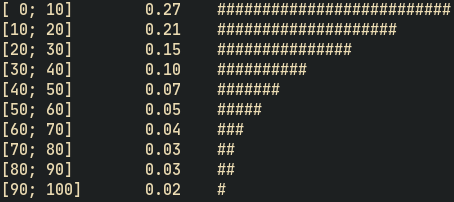
\includegraphics[scale=0.5]{log}\end{center}


\subsection{Метод Аренса для генерування гамма-розподілу порядку}
Таблиця інтервалів та частот попадання чисел для Методу логарифму для генерування показового розподілу при $10,000,000$ псевдовипадково знегеровних чисел:

\begin{table}[ht]
\centering % used for centering table
\begin{tabular}{c c} % centered columns (4 columns)
  Інтервал & Частота \\\relax
[ 0; 10] & 0.03 \\\relax
[10; 20] & 0.08 \\\relax
[20; 30] & 0.26 \\\relax
[30; 40] & 0.31 \\\relax
[40; 50] & 0.11 \\\relax
[50; 60] & 0.04 \\\relax
[60; 70] & 0.02 \\\relax
[70; 80] & 0.01 \\\relax
[80; 90] & 0.01 \\\relax
[90; 100] & 0.01
\end{tabular}
\end{table}
Фотографія гістограмми програми у стандартний поток виводу:
\begin{center}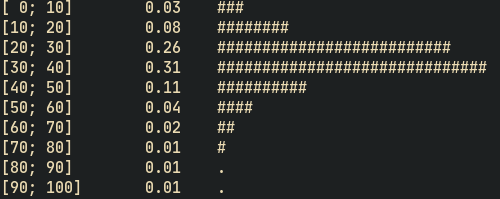
\includegraphics[scale=0.5]{arens}\end{center}

\end{document}
